\documentclass{scrartcl}
\usepackage{etoolbox}
\usepackage{bbm}
\usepackage{amsmath}
\usepackage{amssymb}
\usepackage{mathabx}
\usepackage{graphicx}
\usepackage{float}
\usepackage{parskip}
\usepackage{indentfirst}
\usepackage{fancyhdr}
\usepackage{hyperref}
\pagestyle{fancy}
\usepackage{subcaption}
\setlength{\parskip}{0em}
\setlength{\parindent}{2em}

%-----------------------------------------------------------------------------
\begin{document}





%-----------------------------------------------------------------------------
% header
\lhead{Huwenbo Shi (603-778-363) shihuwenbo@ucla.edu}

% title
\newcommand*{\TitleFont}{
      \usefont{\encodingdefault}{\rmdefault}{b}{n}
      \fontsize{16}{20}
      \selectfont}
\newcommand*{\AuthorFont}{
      \usefont{\encodingdefault}{\rmdefault}{r}{n}
      \fontsize{12}{20}
      \selectfont}
\title{\TitleFont Biomath 210 Homework 5}
\author{\AuthorFont Huwenbo Shi (603-778-363) shihuwenbo@ucla.edu}
\maketitle

\newcommand*{\argmin}{\operatornamewithlimits{argmin}\limits}
\newcommand*{\argmax}{\operatornamewithlimits{argmax}\limits}
\newcommand{\tr}{\mathrm{tr}}
\newcommand{\dom}{\mathrm{dom}}
\newcommand{\E}{\mathrm{E}}
\newcommand{\prox}{\mathrm{prox}}
\newcommand{\epi}{\mathrm{epi}}
\def\mb#1{\mathbf{#1}}

%-----------------------------------------------------------------------------

\section*{Problem 6.3}

Let $\pi_i(\pmb{\theta}) = {\exp(\mb{x}_i^*\pmb{\theta}) \over {1 + \exp(\mb{x}_i^*\pmb{\theta})}}$ be the success probability of the $i$-th trial. Then the likelihood
of the data $\mb{x}_1, \dotsc, \mb{x}_m$ is
\begin{equation}
    L(\pmb{\theta}) = \prod_{i=1}^m \left[ {\exp(\mb{x}_i^*\pmb{\theta}) \over {1 + \exp(\mb{x}_i^*\pmb{\theta})}} \right]^{y_i}
                                    \left[ {1 \over {1 + \exp(\mb{x}_i^*\pmb{\theta})}} \right]^{(1-y_i)},
\end{equation}
which has the log-likelihood
\begin{equation}
    \ell(\pmb{\theta}) = \sum_{i=1}^m [y_i \mb{x}_i^*\pmb{\theta} - \ln(1 + \exp(\mb{x}_i^*\pmb{\theta})) ].
\end{equation}
Let $f_i(\pmb{\theta}) = y_i \mb{x}_i^*\pmb{\theta} - \ln(1 + \exp(\mb{x}_i^*\pmb{\theta}))$, then
\begin{equation}
\nabla f_i(\pmb{\theta}) = y_i \mb{x}_i - {\exp(\mb{x}_i^*\pmb{\theta}) \over {1 + \exp(\mb{x}_i^*\pmb{\theta})}} \mb{x}_i
                                        = [y_i-\pi_i(\pmb{\theta})] \mb{x}_i .
\end{equation}
Therefore, the score vector is
\begin{equation}
\nabla \ell(\pmb{\theta}) = \sum_{i=1}^m [y_i-\pi_i(\pmb{\theta})] \mb{x}_i.
\end{equation}

To derive the observed information matrix, we find
\begin{equation}
    { \partial \over \partial \pmb{\theta}_j } f_i (\pmb{\theta})
    = y_i x_{ij} - {\exp(\mb{x}_i^*\pmb{\theta}) \over {1+\exp(\mb{x}_i^*\pmb{\theta})}}x_{ij},
\end{equation}
and
\begin{equation}
    \begin{split}
    { \partial^2 \over \partial \pmb{\theta}_j \partial \pmb{\theta}_k} f_i (\pmb{\theta})
    & = - \left[
        { {(1+\exp(\mb{x}_i^*\pmb{\theta}))\exp(\mb{x}_i^*\pmb{\theta})x_{ik} - \exp(\mb{x}_i^*\pmb{\theta})\exp(\mb{x}^*\pmb{\theta})x_{ik}}
          \over
          {(1+\exp(\mb{x}_i^*\pmb{\theta}))^2}}
        \right]x_{ij} \\
    & = - {\exp(\mb{x}_i^*\pmb{\theta}) \over {1+\exp(\mb{x}_i^*\pmb{\theta})}}
        \left[
        x_{ik} - { {\exp(\mb{x}^*\pmb{\theta})} \over {1+\exp(\mb{x}_i^*\pmb{\theta})}} x_{ik}
        \right] x_{ij} \\
    & = -\pi_i [ \pmb{\theta}) (1-\pi_i(\pmb{\theta}) ] x_{ij}x_{ik} .
    \end{split}
\end{equation}
So, $\partial^2 f_i(\pmb{\theta}) = -\pi_i(\pmb{\theta}) [ 1-\pi_i(\pmb{\theta}) ] \mb{x}_i\mb{x}_i^*$, and
$\partial^2 \ell(\pmb{\theta}) = -\sum_{i=1}^m \pi_i(\pmb{\theta}) [ 1-\pi_i(\pmb{\theta}) ] \mb{x}_i\mb{x}_i^*$.
The observed information matrix is therefore,
$-\partial^2 \ell(\pmb{\theta}) = \sum_{i=1}^m \pi_i(\pmb{\theta}) [ 1-\pi_i(\pmb{\theta}) ] \mb{x}_i\mb{x}_i^*$.

%-----------------------------------------------------------------------------

\section*{Problem 6.6 (?)}

First, we derive the majorization for $\sqrt{u^2+\epsilon}-\sqrt{\epsilon}$. Let $f(v) = \sqrt{v+\epsilon} - \sqrt{\epsilon}$.
Because $f(v)$ is a concave function, it satisfies the supporting hyperplane inequality
\begin{equation}
\sqrt{v+\epsilon}-\sqrt{\epsilon} \le \sqrt{w+\epsilon} - \sqrt{\epsilon} + {1 \over 2 \sqrt{w+\epsilon}}(v-w).
\label{eqn:concave_ineq}
\end{equation}
Set $v = u^2$ and $w = u_n^2$, we have
\begin{equation}
\sqrt{u^2+\epsilon}-\sqrt{\epsilon} \le \sqrt{u_n^2+\epsilon}-\sqrt{\epsilon} + {1 \over 2 \sqrt{u_n^2+\epsilon}}(u^2-u_n^2).
\end{equation}
Equality holds when $u = u_n$.

Next, we derive the majorization for $\sqrt{u_+^2+\epsilon}-\sqrt{\epsilon}$. For $u_n = 0$, we have the inequality
$\sqrt{u_+^2+\epsilon}-\sqrt{\epsilon} \le {1 \over 2 \sqrt{\epsilon}}u_+^2$ by substituting $v=u_+^2$ and $w=0$ in \eqref{eqn:concave_ineq}.
Since $u^2 \ge u_+^2$, we have $\sqrt{u_+^2+\epsilon}-\sqrt{\epsilon} \le {1 \over 2 \sqrt{\epsilon}}u^2$. Clearly, equality holds when $u=u_n=0$.

%-----------------------------------------------------------------------------

\section*{Problem 6.8}

First, we find the optimal $\mb{D}$ by minimizing $\|\mb{S}-\mb{F}\mb{F}^*-\mb{D}\|_F^2$ when $\mb{F}$ is fixed. We notice that
\begin{equation}
\begin{split}
& \|\mb{S}-\mb{F}\mb{F}^*-\mb{D}\|_F^2  = \tr [(\mb{S}-\mb{F}\mb{F}^*-\mb{D})^*(\mb{S}-\mb{F}\mb{F}^*-\mb{D})] \\
& = \tr(\mb{S}\mb{S}) - 2\tr(\mb{S}\mb{F}\mb{F}^*) - 2\tr(\mb{S}\mb{D}) + 2\tr(\mb{D}\mb{F}\mb{F}^*) + \tr(\mb{D}\mb{D}) + \tr(\mb{F}\mb{F}^*\mb{F}\mb{F}^*) \\
& = - 2\tr(\mb{S}\mb{D}) + 2\tr(\mb{D}\mb{F}\mb{F}^*) + \tr(\mb{D}\mb{D}) + c \\
& = -2 \sum_i \mb{S}_{ii}\mb{d}_i + 2 \sum_i (\mb{F}\mb{F}^*)_{ii}\mb{d}_i + \mb{d}^*\mb{d} + c,
\end{split}
\end{equation}
where $c$ is a constant and $\mb{D} = \text{diag}(\mb{d})$. Setting each component of the gradient ($-2\mb{S}_{ii}+2(\mb{F}\mb{F}^*)_{ii}+2\mb{d}_i$) to 0, we get
$\mb{d}_i = \mb{S}_{ii} - (\mb{F}\mb{F}^*)_{ii}$. Therefore, when $\mb{F}$ is fixed, the optimal diagonal matrix $\mb{D}$ satisfies
$\mb{D}_{ii} = \mb{S}_{ii} - (\mb{F}\mb{F}^*)_{ii}$.

Next, we fix $\mb{D}$ and minimize the objective over $\mb{F}$. Let $\mb{N} = \mb{F}\mb{F}^*$, we first minimize the objective
$f(\mb{N}) = - 2\tr(\mb{S}\mb{N}) + 2\tr(\mb{D}\mb{N}) + \tr(\mb{N}\mb{N}) + e$, where $e$ is a constant, over $\mb{N}$ with the constraint that
$\mb{N}$ is positive semi-definite and $\text{rank}(\mb{N}) \le r$. This problem is equivalent to finding the best rank $r$ approximation of $\mb{S}-\mb{D}$ because
the objective can be written as $f(\mb{N}) = \tr(\mb{N}\mb{N})-2\tr[(\mb{S}-\mb{D})\mb{N}]+\tr[(\mb{S}-\mb{D})^*(\mb{S}-\mb{D})]+b=\|\mb{N}-(\mb{S}-\mb{D})\|_F^2+b$,
where $b$ is a constant. From \textbf{Proposition 7.2.3}, an analytical solution for $\mb{N}$ is
\begin{equation}
\mb{N} = \mb{F}\mb{F}^* = \sum_{i=1}^r \max\{\sigma_i,0\} \mb{u}_i \mb{u}_i^*,
\label{eqn:n_sln}
\end{equation}
where $\sigma_i$ and $\mb{u}_i$ are the eigenvalues and eigenvectors of the ordered spectral decomposition $\mb{S}-\mb{D} = \mb{U}\mb{\Sigma}\mb{U}^*$.
Solution $\mb{F}$ to the equality in Equation \eqref{eqn:n_sln} is not unique. One can set $\mb{F} = \sum_{i=1}^r \sqrt{\max\{\sigma_i,0\}} \mb{u}_i \mb{u}_i^*$
Alternatively, one can set the $i$-th column of the first $r$ columns of $\mb{F}$ to be $\sqrt{\max\{\sigma_i,0\}} \mb{u}_i$ and $\mb{0}$ for the rest.
Both solutions satisfy the equality in Equation \eqref{eqn:n_sln}.

%-----------------------------------------------------------------------------

\section*{Problem 6.13}

We first write the likelihood of the data
\begin{equation}
L(\mb{M},\mb{U},\mb{V})
= \prod_{i=1}^k { {\exp [-{1 \over 2} \tr( \mb{V}^{-1}(\mb{X}_i-\mb{M})^*\mb{U}^{-1}(\mb{X}_i-\mb{M}) )]}
                  \over {(2\pi)^{{np} \over 2} \det(\mb{V})^{n \over 2} \det(\mb{U})^{p \over 2}}
                },
\end{equation}
with log-likelihood
\begin{equation}
\begin{split}
\ell (\mb{M},\mb{U},\mb{V}) & = \sum_{i=1}^k
 \left\lbrace -{1 \over 2} \tr [ \mb{V}^{-1}(\mb{X}_i-\mb{M})^*\mb{U}^{-1}(\mb{X}_i-\mb{M}) ] \right\rbrace \\
& {\;\;\;\;} - k \ln [ (2\pi)^{{np} \over 2} ] -  k {n \over 2} \ln \det(\mb{V}) - k {p \over 2} \ln \det(\mb{U}) \\
& = \sum_{i=1}^k \left[ -{1 \over 2} \tr(\mb{V}^{-1}\mb{X}_i^*\mb{U}^{-1}\mb{X}_i)
     + \tr(\mb{V}^{-1}\mb{X}_i^*\mb{U}^{-1}\mb{M}) - {1 \over 2} \tr(\mb{V}^{-1}\mb{M}^*\mb{U}^{-1}\mb{M}) \right] \\
& {\;\;\;\;} - k \ln [ (2\pi)^{{np} \over 2} ] -  k {n \over 2} \ln \det(\mb{V}) - k {p \over 2} \ln \det(\mb{U}) .
\end{split}
\end{equation}

We first estimate the mean $\mb{M}$. Taking the derivative with respect to $\mb{M}$ and setting it to zero, we get
\begin{equation}
\begin{split}
0 = \sum_{i=1}^k \mb{V}^{-1}\mb{X}_i^*\mb{U}^{-1}-\mb{V}\mb{M}\mb{U}^{-1} 
  = \mb{V}^{-1} \left( \sum_{i=1}^k \mb{X}_i - k\mb{M} \right) \mb{U}^{-1}
\end{split}
\end{equation}
Solving for $\mb{M}$, we get $\mb{M} = {1 \over k} \sum_{i=1}^k \mb{X}_i$.

Next, we fix $\mb{V}$, and maximize the log-likelihood over $\mb{U}$. Taking the derivative with respect to $\mb{U}^{-1}$ and setting it to zero, we get
\begin{equation}
0 = - \sum_{i=1}^k \left( {1 \over 2} \mb{X}_i\mb{V}^{-1}\mb{X}_i^* - \mb{M}\mb{V}^{-1}\mb{X}_i^* + {1 \over 2}\mb{M}\mb{V}^{-1}\mb{M} \right)
                  - {kp \over 2} \mb{U}
\end{equation}
Solving for $\mb{U}$, we get $\mb{U} = {1 \over kp}\sum_{i=1}^k (\mb{X}_i-\mb{M})^*\mb{V}^{-1}(\mb{X}_i-\mb{M})$.

Finally, we fix $\mb{U}$, and maximize the log-likelihood over $\mb{V}$. Similarly, we set the derivative with respect to $\mb{V}^{-1}$ to 0, and get
\begin{equation}
0 = - \sum_{i=1}^k \left( {1 \over 2} \mb{X}_i\mb{U}^{-1}\mb{X}_i^* - \mb{M}\mb{U}^{-1}\mb{X}_i^* + {1 \over 2}\mb{M}\mb{U}^{-1}\mb{M} \right)
                  - {kn \over 2} \mb{V}
\end{equation}
Solving for $\mb{V}$, we get $\mb{V} = {1 \over kn}\sum_{i=1}^k (\mb{X}_i-\mb{M})^*\mb{U}^{-1}(\mb{X}_i-\mb{M})$.

%-----------------------------------------------------------------------------

\section*{Problem 6.14}

For the mixture of $r$ Gaussian distributions, the density of $\mb{y}$ is $\Pr(\mb{y}) = \sum_{j=1}^r \pi_j f(\mb{y}|\pmb{\mu}_j, \pmb{\Omega})$.
The likelihood is therefore,
\begin{equation}
L(\pmb{\Theta}) = 
\prod_{i=1}^m \left[  \sum_{j=1}^r \pi_j f(\mb{y}_i|\pmb{\mu}_j, \pmb{\Omega}) \right],
\end{equation}
with log-likelihood
\begin{equation}
\begin{split}
\ell (\pmb{\Theta}) & =
\sum_{i=1}^m \ln \left[  \sum_{j=1}^r \pi_j f(\mb{y}_i|\pmb{\mu}_j, \pmb{\Omega}) \right] \\
& = \sum_{i=1}^m \ln
\left\lbrace
\sum_{j=1}^r \pi_j {1 \over ({2\pi})^{p \over 2} \det(\pmb{\Omega})^{1 \over 2}} \exp[-{1\over 2}(\mb{y}_i-\pmb{\mu}_j)^*\pmb{\Omega}^{-1}(\mb{y}_i-\pmb{\mu}_j)]
\right\rbrace,
\end{split}
\end{equation}
where $\pmb{\Theta} = (\pmb{\mu}_j, \pmb{\Omega})$ represents the parameters.
We maximize the log-likelihood with the constraint $\sum_{j=1}^r \pi_j = 1$, which entails the Lagrangian,
\begin{equation}
\sum_{i=1}^m \ln
\left\lbrace
\sum_{j=1}^r \pi_j {1 \over ({2\pi})^{p \over 2} \det(\pmb{\Omega})^{1 \over 2}} \exp[-{1\over 2}(\mb{y}_i-\pmb{\mu}_j)^*\pmb{\Omega}^{-1}(\mb{y}_i-\pmb{\mu}_j)]
\right\rbrace + \lambda \sum_{j=1}^r \pi_j - \lambda.
\end{equation}
Following Example (1.3), we obtain the minorization
\begin{equation}
\begin{split}
& \sum_{i=1}^m \ln \left[  \sum_{j=1}^r \pi_j f(\mb{y}_i|\pmb{\mu}_j, \pmb{\Omega}) \right] + \lambda \sum_{j=1}^r \pi_j - \lambda \\ 
& \ge \sum_{i=1}^m
    \sum_{j=1}^r
        { w_{nij} }
        \ln \left\lbrace
            { 1 \over w_{nij}}
            \pi_j {1 \over ({2\pi})^{p \over 2} \det(\pmb{\Omega})^{1 \over 2}} \exp[-{1\over 2}(\mb{y}_i-\pmb{\mu}_j)^*\pmb{\Omega}^{-1}(\mb{y}_i-\pmb{\mu}_j)]
        \right\rbrace + \lambda \sum_{j=1}^r \pi_j - \lambda \\
& = \sum_{i=1}^m \sum_{j=1}^r { w_{nij} }
    \left[ \ln \pi_j - {1 \over 2} \ln \det(\pmb{\Omega}) -{1\over 2}(\mb{y}_i-\pmb{\mu}_j)^*\pmb{\Omega}^{-1}(\mb{y}_i-\pmb{\mu}_j) \right] 
    + \lambda \sum_{j=1}^r \pi_j - \lambda + c_n,
\end{split}
\label{eqn:p614_obj}
\end{equation}
where $c_n$ is a constant.

Taking derivative with respect to $\pi_j$, and setting it to 0, we get
\begin{equation}
0 = {1 \over \pi_{n+1,j}} \sum_{i=1}^m w_{nij} + \lambda , \; \text{and\;} \pi_{n+1,j} = - {1 \over \lambda} \sum_{i=1}^m w_{nij}.
\end{equation}
Summing over $j$ we get $\sum_{i=1}^r \pi_j = 1 = - {1 \over \lambda} \sum_{i=1}^m \sum_{j=1}^r w_{nij} = - {m \over \lambda}$, which entails
$\lambda = -m$ and that $\pi_{n+1,j} = {1 \over m} \sum_{i=1}^m w_{nij}$.

We update $\pmb{\mu}_j$ and $\pmb{\Omega}$ through block descent. The objective in Equation \eqref{eqn:p614_obj} can be written as
\begin{equation}
\begin{split}
& \sum_{i=1}^m \sum_{j=1}^r { w_{nij} } \ln \pi_j - {m \over 2} \ln \det(\pmb{\Omega}) + \lambda \sum_{j=1}^r \pi_j - \lambda + c_n \\
& - {1\over 2} \sum_{j=1}^r \left[ ( \sum_{i=1}^m w_{nij} \mb{y}_i-\pmb{\mu}_j \sum_{i=1}^m w_{nij})^*\pmb{\Omega}^{-1}
( \sum_{i=1}^m w_{nij} \mb{y}_i-\pmb{\mu}_j \sum_{i=1}^m w_{nij}) \right].
\end{split}
\label{eqn:lagrangian_rewrite}
\end{equation}
The last term of the above equation entails the update for $\pmb{\mu}_{n+1,j}$,
\begin{equation}
\pmb{\mu}_{n+1,j} = {1 \over \sum_{i=1}^m w_{nij}}\sum_{i=1}^m w_{nij} \mb{y}_i,
\end{equation}
at which the last term of Equation \eqref{eqn:lagrangian_rewrite} attains its minimum 0.

Next, we fix $\pmb{\mu}_j = \pmb{\mu}_{n+1,j}$.  Taking the derivative with respect to $\pmb{\Omega}^{-1}$, and setting it to 0 yields
\begin{equation}
0 = {m \over 2} \pmb{\Omega} - {1 \over 2} \sum_{j=1}^r \sum_{i=1}^m w_{nij} (\mb{y}_i-\pmb{\mu}_{n+1,j})(\mb{y}_i-\pmb{\mu}_{n+1,j})^* ,
\end{equation}
which entails the update
\begin{equation}
\pmb{\Omega}_{n+1,j} = {1 \over m} \sum_{j=1}^r \sum_{i=1}^m w_{nij} (\mb{y}_i-\pmb{\mu}_{n+1,j})(\mb{y}_i-\pmb{\mu}_{n+1,j})^* .
\end{equation}

%------------------------------------------------------------------------

\section*{Problem 6.15}

Imposing the inverse Wishart prior, we obtain the log-likelihood
\begin{equation}
\begin{split}
\ell (\pmb{\Theta}) & =
\sum_{i=1}^m \ln
\left\lbrace
\sum_{j=1}^r \pi_j {1 \over ({2\pi})^{p \over 2} \det(\pmb{\Omega}_j)^{1 \over 2}} \exp[-{1\over 2}(\mb{y}_i-\pmb{\mu}_j)^*\pmb{\Omega}_j^{-1}(\mb{y}_i-\pmb{\mu}_j)]
\right\rbrace \\
& \;\;\;\; - \sum_{j=1}^r \left[ {a \over 2} \ln \det \pmb{\Omega}_j + {b \over 2} \tr(\pmb{\Omega}_j^{-1}\mb{S}_j) \right].
\end{split}
\end{equation}
With the constraint $\sum_{j=1}^r \pi_j = 1$, the Lagrangian becomes
\begin{equation}
\begin{split}
& \sum_{i=1}^m \ln
\left\lbrace
\sum_{j=1}^r \pi_j {1 \over ({2\pi})^{p \over 2} \det(\pmb{\Omega}_j)^{1 \over 2}} \exp[-{1\over 2}(\mb{y}_i-\pmb{\mu}_j)^*\pmb{\Omega}_j^{-1}(\mb{y}_i-\pmb{\mu}_j)]
\right\rbrace \\
& - \sum_{j=1}^r \left[ {a \over 2} \ln \det \pmb{\Omega}_j + {b \over 2} \tr(\pmb{\Omega}_j^{-1}\mb{S}_j) \right] + \lambda \sum_{j=1}^r \pi_j - \lambda.
\end{split}
\end{equation}
Similarly, we have the minorization
\begin{equation}
\begin{split}
& \sum_{i=1}^m \sum_{j=1}^r { w_{nij} }
    \left[ \ln \pi_j - {1 \over 2} \ln \det(\pmb{\Omega}_j) -{1\over 2}(\mb{y}_i-\pmb{\mu}_j)^*\pmb{\Omega}_j^{-1}(\mb{y}_i-\pmb{\mu}_j) \right] \\
& - \sum_{j=1}^r \left[ {a \over 2} \ln \det \pmb{\Omega}_j + {b \over 2} \tr(\pmb{\Omega}_j^{-1}\mb{S}_j) \right] + \lambda \sum_{j=1}^r \pi_j - \lambda + c_n
\end{split}
\end{equation}

The derivative of the surrogate function with respect to $\pi_j$ doesn't change, so
\begin{equation}
0 = {1 \over \pi_{n+1,j}} \sum_{i=1}^m w_{nij} + \lambda , \; \text{and\;} \pi_{n+1,j} = - {1 \over \lambda} \sum_{i=1}^m w_{nij}.
\end{equation}

Similar to Equation \eqref{eqn:lagrangian_rewrite}, the Lagrangian can also be written as
\begin{equation}
\begin{split}
& \sum_{i=1}^m \sum_{j=1}^r { w_{nij} } \ln \pi_j - {1 \over 2} \sum_{i=1}^m \sum_{j=1}^r w_{nij} \ln \det(\pmb{\Omega}_j) + \lambda \sum_{j=1}^r \pi_j - \lambda + c_n
- \sum_{j=1}^r \left[ {a \over 2} \ln \det \pmb{\Omega}_j + {b \over 2} \tr(\pmb{\Omega}_j^{-1}\mb{S}_j) \right] \\
& - {1\over 2} \sum_{j=1}^r \left[ ( \sum_{i=1}^m w_{nij} \mb{y}_i-\pmb{\mu}_j \sum_{i=1}^m w_{nij})^*\pmb{\Omega}_j^{-1}
( \sum_{i=1}^m w_{nij} \mb{y}_i-\pmb{\mu}_j \sum_{i=1}^m w_{nij}) \right].
\end{split}
\end{equation}
The last term of the equation above entails the same update for $\pmb{\mu}_j$,
\begin{equation}
\pmb{\mu}_{n+1,j} = {1 \over \sum_{i=1}^m w_{nij}}\sum_{i=1}^m w_{nij} \mb{y}_i,
\end{equation}
Taking $\mb{S}_j = \mb{S}$ for all $j$ and $\pmb{\mu}_j = \pmb{\mu}_{n+1,j}$, and setting the derivative of the Lagrangian with respect to
$\pmb{\Omega}_j^{-1}$ to 0, we get
\begin{equation}
0 = {1 \over 2} \sum_{i=1}^m w_{nij} \pmb{\Omega}_j + {a \over 2} \pmb{\Omega}_j - {b \over 2} \mb{S}_j
-{1 \over 2} \sum_{i=1}^m w_{nij}(\mb{y}_i-\pmb{\mu}_{n+1,j})(\mb{y}_i-\pmb{\mu}_{n+1,j})^*.
\end{equation}
Solving for $\pmb{\Omega}_j$, we obtain
\begin{equation}
\begin{split}
\pmb{\Omega}_j & = {{b \mb{S}} \over {\sum_{i=1}^m w_{nij}+a}}
+ { {\sum_{i=1}^m w_{nij}(\mb{y}_i-\pmb{\mu}_{n+1,j})(\mb{y}_i-\pmb{\mu}_{n+1,j})^*} \over {\sum_{i=1}^m w_{nij}+a}} \\
& = {a \over {\sum_{i=1}^m w_{nij}+a}} \left( {b \over a} \mb{S} \right)
+ { {\sum_{i=1}^m w_{nij}} \over {\sum_{i=1}^m w_{nij}+a} } \tilde{\pmb{\Omega}}_{n+1,j},
\end{split}
\end{equation}
where
\begin{equation}
\tilde{\pmb{\Omega}}_{n+1,j} = {1 \over {\sum_{i=1}^m w_{nij}}} {\sum_{i=1}^m w_{nij}(\mb{y}_i-\pmb{\mu}_{n+1,j})(\mb{y}_i-\pmb{\mu}_{n+1,j})^*}.
\end{equation}


%---------------------------------------------------------------------------------

\section*{Problem 6.16}

We consider the model
\begin{equation}
\mb{y} \sim N\left(\left( \begin{array}{c}
                            \mb{x}_1^* \\
                            \vdots \\
                            \mb{x}_m^*
                          \end{array}
                   \right) \pmb{\beta},
                   \sigma_1^2 \mb{I} + \sigma_2^2
                   \left(
                   \begin{array}{ccc}
                       t_1    & \cdots & 0 \\
                       \vdots & \ddots & \vdots \\
                       0      & \cdots & t_m
                   \end{array}
                   \right)                    
                  \right).
\end{equation}
To create simulations, I draw $\mb{x}_i \in \mb{R}^p$ and $\pmb{\beta} \in \mb{R}^p$ randomly from the uniform distribution (i.e. the rand function in Matlab),
and $\mb{y}$ from the normal distribution shown above. I set $p=10$, $m=100$, and $t_i = 0.01*i$. I created 100 set of simulations in total, and I report the
mean and standard errors of $\hat{\sigma}_1^2$, $\hat{\sigma}_2^2$, and $\hat{\sigma}_1^2 \over {\hat{\sigma}_1^2+\hat{\sigma}_1^2}$. I also include a figure
showing the convergence of the objective. Overall, I observe that the algorithm consistently underestimates $\sigma_1$. But the estimation for $\sigma_2$ and
the ratio $\sigma_1^2 \over {\sigma_1^2+\sigma_2^2}$ is less biased.

\begin{table}[htb]
        \centering
        \begin{tabular}{| l | l | l | l | l | l |}
                \hline
                $\sigma_1^2$ & $\hat{\sigma}_1^2$ (s.e.) & $\sigma_2^2$ & $\hat{\sigma}_2^2$ (s.e.) & $\sigma_1^2 \over {\sigma_1^2+\sigma_2^2}$ & $\hat{\sigma}_1^2 \over {\hat{\sigma}_1^2+\hat{\sigma}_2^2}$ (s.e.) \\ \hline
                2.0 & 1.579 (0.066) & 2.0 & 2.320 (0.173) & 0.500 & 0.472 (0.027) \\ \hline                
                2.0 & 1.537 (0.086) & 4.0 & 4.360 (0.203) & 0.333 & 0.295 (0.020) \\ \hline
                2.0 & 1.559 (0.104) & 6.0 & 6.197 (0.291) & 0.250 & 0.246 (0.021) \\ \hline
                2.0 & 1.591 (0.118) & 8.0 & 8.327 (0.347) & 0.200 & 0.198 (0.019) \\ \hline        
                4.0 & 3.286 (0.120) & 2.0 & 2.648 (0.238) & 0.667 & 0.611 (0.029) \\ \hline        
                6.0 & 4.977 (0.165) & 2.0 & 2.680 (0.285) & 0.750 & 0.700 (0.029) \\ \hline        
                8.0 & 6.329 (0.216) & 2.0 & 3.660 (0.407) & 0.800 & 0.692 (0.030) \\ \hline        
        \end{tabular}
        \caption{Simulated and estimated variance components}
        \label{tbl:param_est}
\end{table}

\begin{figure}[H]
  \begin{minipage}[b]{0.3\textwidth}
    \centering
    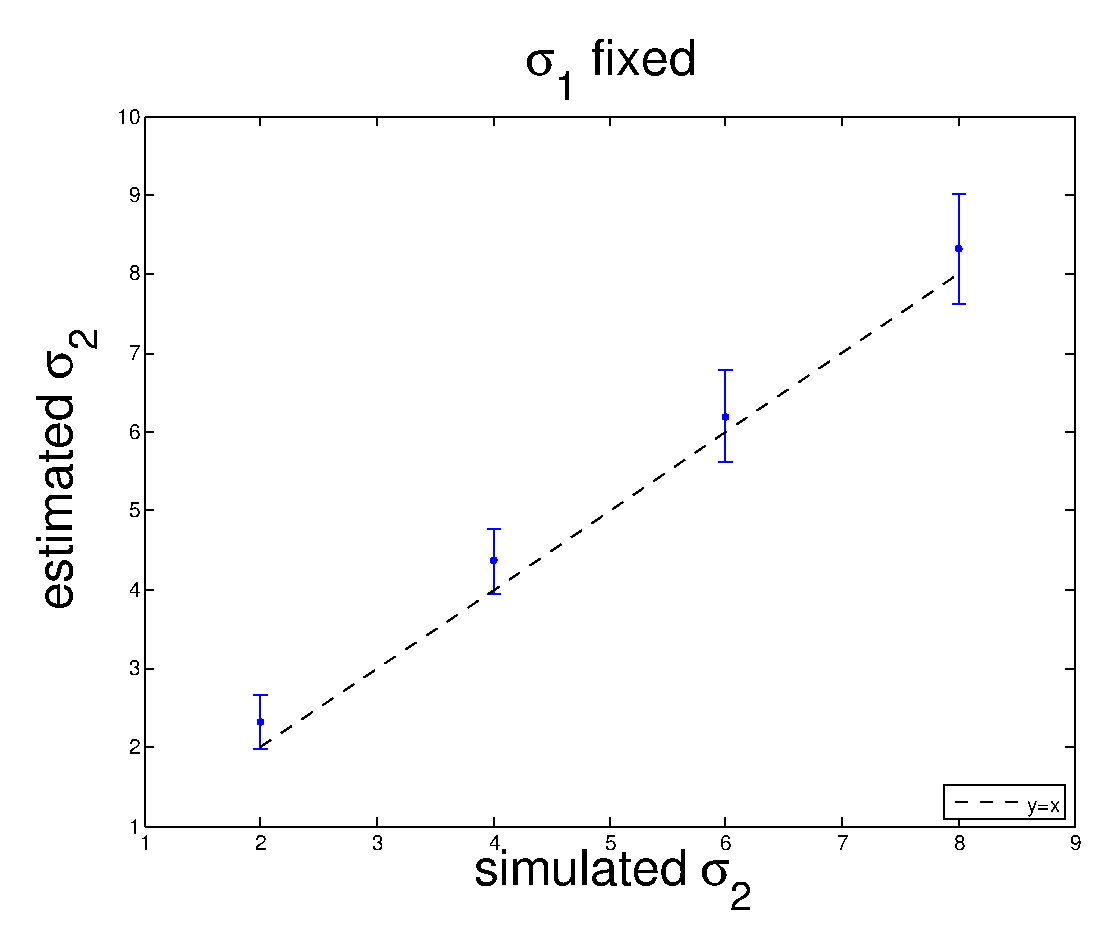
\includegraphics[scale=0.26]{s1_fixed.eps}
  \end{minipage}
  \quad
  \begin{minipage}[b]{0.3\textwidth}
    \centering
    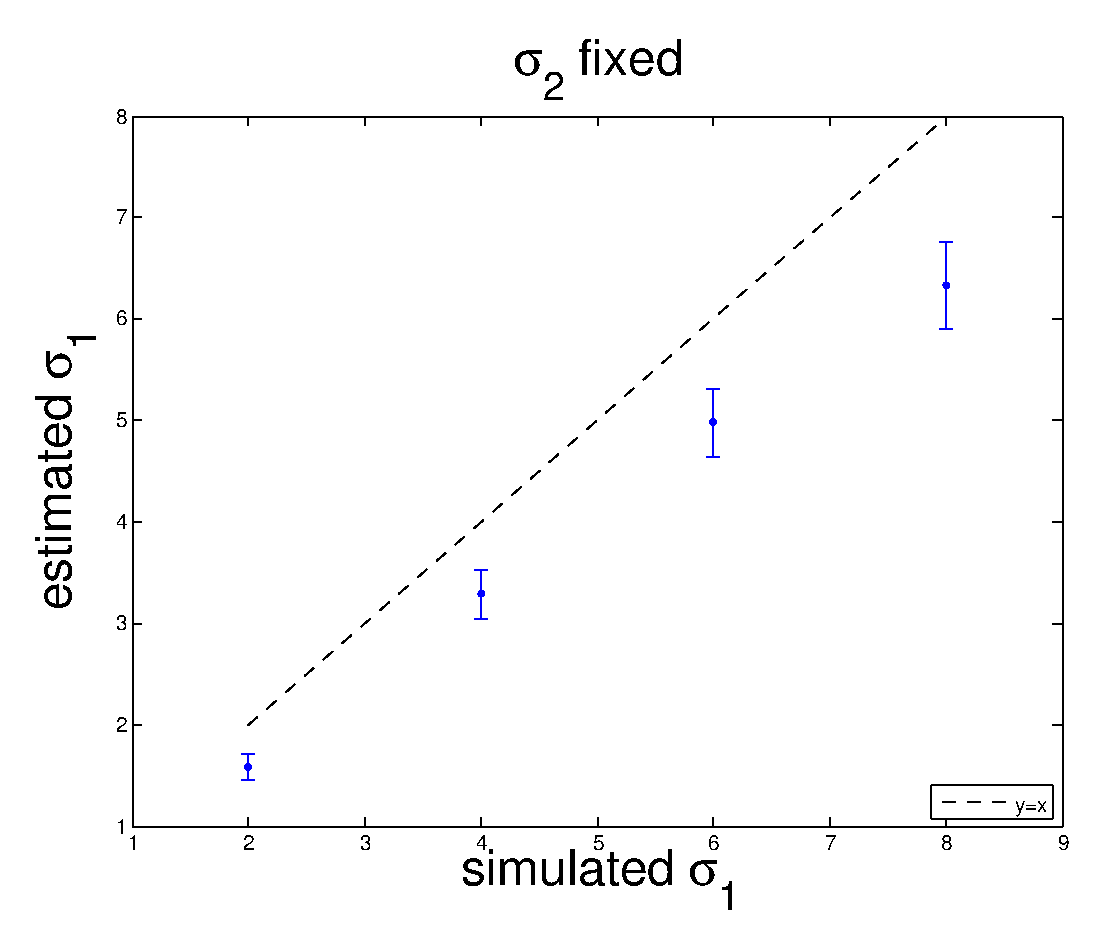
\includegraphics[scale=0.26]{s2_fixed.eps}
  \end{minipage}
  \quad
  \begin{minipage}[b]{0.3\textwidth}
    \centering
    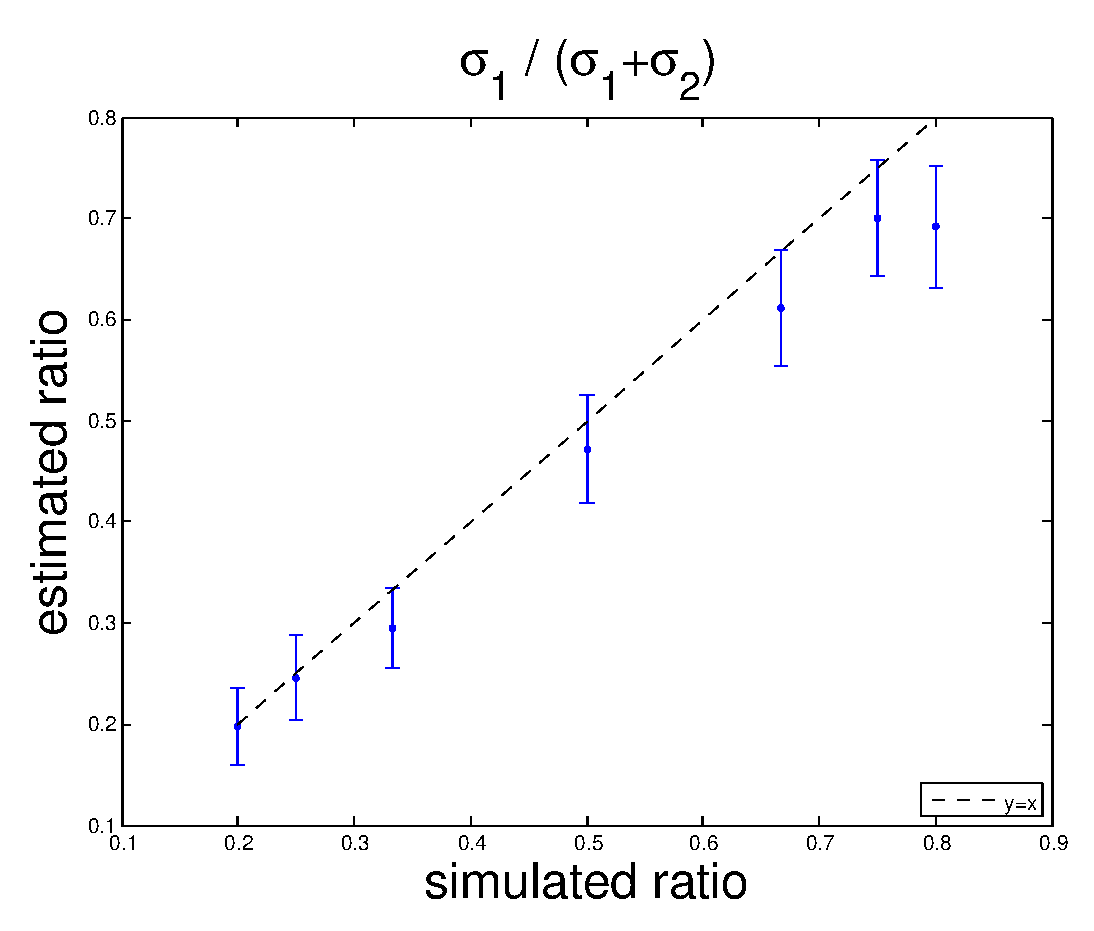
\includegraphics[scale=0.26]{ratio.eps}
  \end{minipage}
  \caption{Estimated variance components vs. simulated variance components. Error bars show 2 $\times$ s.e. on each side.}
  \label{fig:prob16_result}
\end{figure}

\begin{figure}[H]
\centering
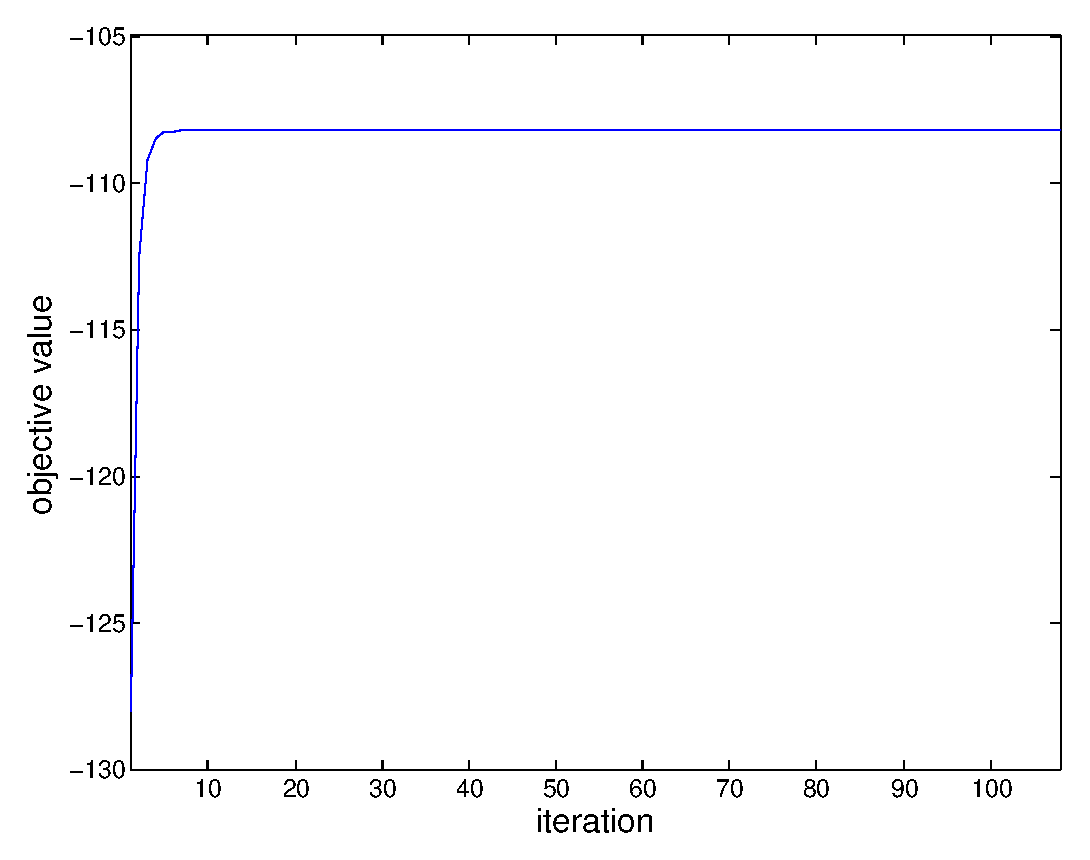
\includegraphics[scale=0.5]{obj_plot.eps}
\caption{Convergence of the objective}
\end{figure}

\subsection*{lmm.m (implements the update 6.8 and 6.10)}

\begin{verbatim}
function [beta, s1, s2, obj_val] = lmm(y, A, V1, V2)
    % initialization
    eps = 10^-4; max_iter = 1000;
    
    s1 = 1.0; s2 = 1.0;
    omega = s1*V1+s2*V2; omega_inv = pinv(omega);
    beta = pinv(A'*omega_inv*A)*A'*omega_inv*y;
    
    obj_val = zeros(max_iter, 1);
    
    % iterate until convergence
    for i=1:max_iter
        
        % compute objval
        obj_val(i) = -0.5*log(det(omega))...
            -0.5*(y-A*beta)'*omega_inv*(y-A*beta);
        
        % compute new sigma
        u = omega_inv*(y-A*beta);
        s1_next = s1*sqrt(u'*V1*u/trace(omega_inv*V1));
        s2_next = s2*sqrt(u'*V2*u/trace(omega_inv*V2));
        
        % compute new omega
        omega = s1_next*V1+s2_next*V2;
        omega_inv = pinv(omega);
        
        % compute new beta
        beta_next = pinv(A'*omega_inv*A)*A'*omega_inv*y;
    
        % check convergence
        dist = norm([s1 s2 beta']-[s1_next s2_next beta']);
        if(dist < eps), break; end
        
        % update parameters
        s1 = s1_next; s2 = s2_next; beta = beta_next;
    end

    obj_val = obj_val(1:i);
end
\end{verbatim}

\subsection*{main.m (generates simulations and tests lmm.m)}

\begin{verbatim}
% simulate data
n = 100;                    % number of simulations
m = 100;                    % number of samples
p = 10;                     % number of dimensions
sigma_1 = 2.0;              % simulated sigma_1
sigma_2 = 4.0;              % simulated sigma_2
sim_rec = zeros(n, 5);      % record simulation result

% simulate data and estimate sigma_1 and sigma_2
for i=1:n
    
    % simulate y
    beta = rand(p, 1);       % beta vector for simulation
    A  = rand(m, p);         % measurement matrix
    V1 = eye(m);             % variance component 1
    V2 = diag(1:m)/100;      % variance component 2 (time)
    y  =  mvnrnd(A*beta, sigma_1*V1+sigma_2*V2)';
    
    % esimate beta, sigma_1, and sigma_2
    [beta_est, s1_est, s2_est, obj_val] = lmm(y, A, V1, V2);
    if(i == 1)
        figure('visible', 'off'); plot(obj_val, 'b-');
        xlim([1 size(obj_val,1)]); xlabel('iteration');
        ylabel('objective value'); set(gca,'FontSize',12)
        print('prob_16_obj','-depsc','-r0');
    end
    
    % record result
    sim_rec(i,:) = [sigma_1 s1_est sigma_2 s2_est norm(beta-beta_est)];
end

% print summary
fprintf('s1: %.3f\n', sigma_1);
fprintf('estimated s1: %.3f %.3f\n', mean(sim_rec(:,2)), ...
    sqrt(var(sim_rec(:,2))/n));

fprintf('\n');

fprintf('s2: %.2f\n', sigma_2);
fprintf('estimated s2: %.3f %.3f\n', mean(sim_rec(:,4)), ...
    sqrt(var(sim_rec(:,4))/n));

fprintf('\n');

fprintf('s1/(s1+s2): %.3f\n', sigma_1/(sigma_1+sigma_2));
fprintf('estimated s1/(s1+s2): %.3f %.3f\n', ...
    mean(sim_rec(:,2)./(sim_rec(:,2)+sim_rec(:,4))),...
    sqrt(var(sim_rec(:,2)./(sim_rec(:,2)+sim_rec(:,4)))/n));
\end{verbatim}

%---------------------------------------------------------------------------------

\section*{Problem 6.17}

In this problem, we assume that $\mb{A}$ is a positive definite matrix. Let
\begin{equation}
f(\mb{x}, \mb{A}) = \sup_{\mb{y}} \left[ \mb{x}^*\mb{y} - {1 \over 2} \mb{y}^*\mb{A}\mb{y} \right].
\end{equation}
Since $\mb{A}$ is positive definite, the function inside the supremum is strictly convex. Based on Example 3.4.2, we know that the maximum is attained at
$\mb{y} = \mb{A}^{-1}\mb{x}$, which yields $f(\mb{x}, \mb{A}) = {1 \over 2} \mb{x}^*\mb{A}^{-1}\mb{x}$.
Because the Fenchel conjugate is convex, we conclude that the map $(\mb{x},\mb{A}) \rightarrow {1 \over 2} \mb{x}^*\mb{A}^{-1}\mb{x}$ is convex.

%---------------------------------------------------------------------------------

\section*{Problem 6.19}

First, we show that $\mb{v}_j$ lie on the surface of the unit sphere in $\mb{R}^{c-1}$.
For $j = 1$, $\|\mb{v}_1\| = (c-1)^{-{1 \over 2}} \|\mb{1}\| = (c-1)^{-{1 \over 2}}(c-1)^{1 \over 2} = 1$.
For $2 \le j \le c$, 
\begin{equation}
\begin{split}
\|\mb{v}_j\| & = [ (r\mb{1}+s\mb{e}_{j-1})^*(r\mb{1}+s\mb{e}_{j-1}) ]^{1 \over 2} = [ r^2(c-1) + s^2 + 2rs ]^{1 \over 2} \\
& = \left[ { {(1+\sqrt{c})^2} \over {(c-1)^2} } + {c \over {c-1}} - 2 {\sqrt{c} \over \sqrt{c-1}} {{1+\sqrt{c}} \over {(c-1)^{3 \over 2}}} \right]^{1 \over 2} \\
& = \left[ {{c^2-2c+1} \over {(c-1)^2}} \right]^{1 \over 2} = 1.
\end{split}
\end{equation}
Therefore, all $\mb{v}_j$ lie on the surface of the unit sphere in $\mb{R}^{c-1}$.

To prove equidistance, we first show that the distance between $\mb{v}_1$ and all other $\mb{v}_j$ is the same. We compute the distance between $\mb{v}_1$
and an arbitrary $\mb{v}_k$,
\begin{equation}
\begin{split}
\|\mb{v}_1 - \mb{v}_k\|^2 & = \|\mb{v}_1\|^2+\|\mb{v}_k\|^2 - 2 \mb{v}_1^*\mb{v}_k = 2 - 2 \mb{v}_1^*\mb{v}_k \\
& = 2 - 2 [ r(c-1)^{-{1\over 2}}(c-1)+(c-1)^{-{1\over 2}}s ]\\
& = 2 - 2 \left[ -{{1+\sqrt{c}} \over {c-1}} + {\sqrt{c} \over {c-1}}\right] = 2 + {2 \over {c-1}}.
\end{split}
\end{equation}
Therefore, the distance between $\mb{v}_1$ and all other $\mb{v}_j$ is $\sqrt{2 + {2 \over {c-1}}}$.
Next, we show that the distance between $\mb{v}_j$ and $\mb{v}_k$ for any arbitrary $c \ge j \ge 2$, $c \ge k \ge 2$, and $k \neq j$ are the same.
We compute the distance between $\mb{v}_j$ and $\mb{v}_k$,
\begin{equation}
\begin{split}
\|\mb{v}_j - \mb{v}_k\|^2 & = \|\mb{v}_j\|^2+\|\mb{v}_k\|^2 - 2 \mb{v}_j^*\mb{v}_k = 2 - 2 \mb{v}_j^*\mb{v}_k \\
& = 2 - 2 [r^2(c-2) + 2rs ] \\
& = 2 - 2 \left[ {{1+c+2\sqrt{c}} \over {(c-1)^2}} - {{2(1+\sqrt{c})\sqrt{c}} \over {(c-1)^2}}\right] \\
& = 2 - 2 \left[ {{1-c} \over {(c-1)^2}} \right] = 2 + {2 \over {c-1}}.
\end{split}
\end{equation}
Therefore, the distance between $\mb{v}_j$ and $\mb{v}_k$ are the same.

In conclusion, $\mb{v}_j$ lie on the surface of the unit sphere in $\mb{R}^{c-1}$, and that all vertex pairs are equidistant.

%---------------------------------------------------------------------------------

\section*{Problem 6.20}

We show that for $\mb{R}^{c-1}$ the maximum number of pairwise equidistant points that can be situated is $c$. Let $\mb{x}_0, \cdots, \mb{x}_{c-1} \in \mb{R}^{c-1}$
be the set of pairwise equidistant points such that $\|\mb{x}_i - \mb{x}_j\| = d$ for all pairs of $i \neq j$. Without loss of generality, we subtract $\mb{x}_0$
from each $\mb{x}_i$, resulting in the new set of points $\mb{0}, \mb{x}_1-\mb{x}_0, \cdots, \mb{x}_{c-1}-\mb{x}_0$. Since
$\|\mb{x}_i - \mb{x}_j\| = \|(\mb{x}_i-\mb{x}_0) - (\mb{x}_j-\mb{x}_0)\|=d$, the new set of points are still pairwise equidistant.
Let $\mb{y}_0 = \mb{0}, \cdots, \mb{y}_{c-1} = \mb{x}_{c-1}-\mb{x}_0$ denote the new set of points. For each $i \ge 1$, we have
$\|\mb{y}_i\| = \|\mb{y}_i-\mb{0}\| = \sqrt{\mb{y}_i^*\mb{y}_i} = d$. And for each $i \neq j$, we have $\|\mb{y}_i-\mb{y}_j\| = d$. Since
$\|\mb{y}_i-\mb{y}_j\|^2 = d^2+d^2-2\mb{y}_i^*\mb{y}_j=d^2$ for $i \neq j$, we also have the equality $\mb{y}_i^*\mb{y}_j = {d^2 \over 2}$.
Now we show that the vectors $\mb{y}_1, \cdots, \mb{y}_{c-1}$ are linear independent. Let $a_1, \cdots, a_{c-1}$ be scalars such that
$\sum_{i=1}^{c-1} a_i \mb{y}_i = 0$. Taking the inner product of $\mb{y}_j$ and $\sum_{i=1}^{c-1} a_i \mb{y}_i$ yields the equality
$\mb{y}_j^*(\sum_{i=1}^{c-1} a_i \mb{y}_i) = \sum_{i=1}^{c-1} a_i \mb{y}_i^*\mb{y}_j = a_j d^2 + \sum_{i=1, i \neq j}^{c-1} a_i {d^2 \over 2}= 0$.
Since $d$ is positive, the equality is satisfied only if $a_1 = \cdots = a_{c-1} = 0$. Therefore, the vectors $\mb{y}_1, \cdots, \mb{y}_{c-1}$ are linear
independent and form a basis for $\mb{R}^{c-1}$. In other words, the problem of finding pairwise equidistant points in $\mb{R}^{c-1}$ is equivalent to
finding the basis of $\mb{R}^{c-1}$ on the sphere $\{\mb{x} : \|x\|=d\}$ that satisfies $\|\mb{x}_i-\mb{x}_j\| = d$ for $i \neq j$ and then including the
point $\mb{0}$, which can then be shifted and rotated. Since the number of vectors in the basis for $\mb{R}^{c-1}$ is $c-1$, the number of pairwise equidistant points
that can be situated is $c$. And it's impossible to situate $c+1$ points in $\mb{R}^{c-1}$.


\end{document}